\begin{figure}[t!]
  \centering
  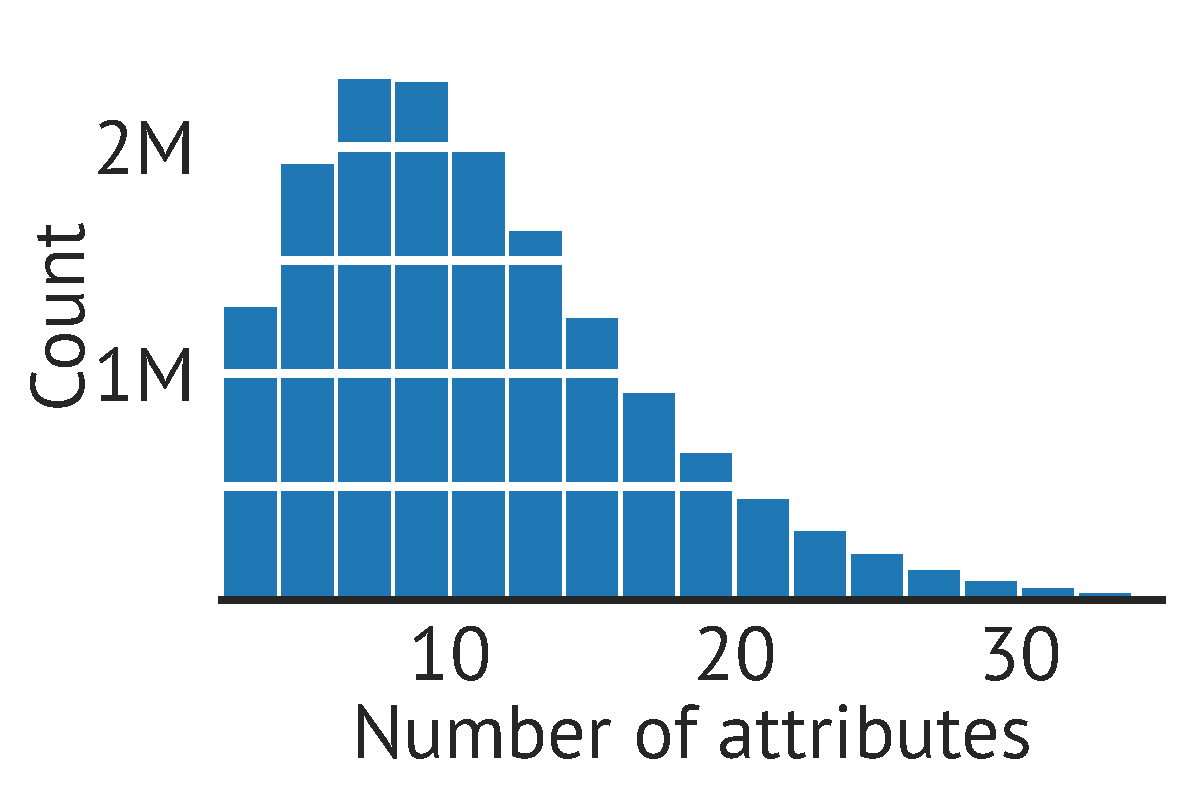
\includegraphics[width=0.6\linewidth]{fig/hist_meals}
%  \vspace*{-8mm}
  \caption{A histogram of the number of foods illustrates the statistical
    challenge of building models to rank from sets. Even in this subset of the
    data, 50k users consume 16M meals in one year. This means when building a
    model to rank meals, a model with unique parameters for every datapoint is
    inefficient: models should share parameters across meals.}
  % \end{minipage}
  % \begin{minipage}[c]{0.49\linewidth}
  %   \centering
  %   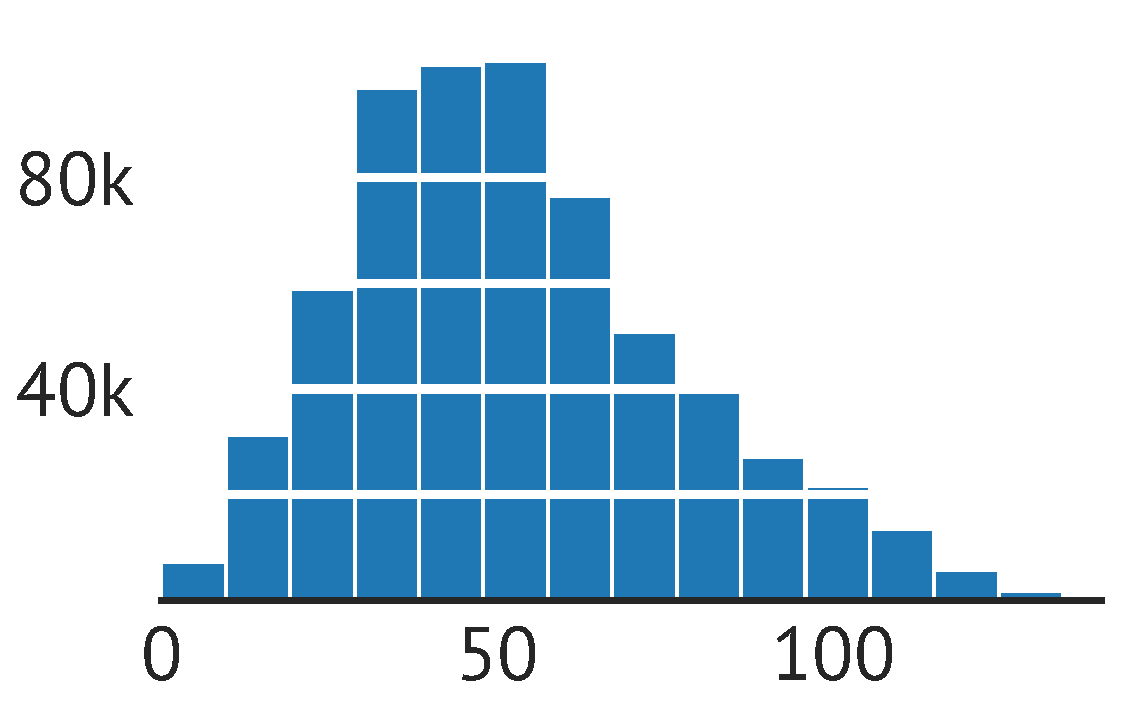
\includegraphics[width=\textwidth]{fig/hist_arxiv}
  %   \vspace*{-8mm}
  %   \caption*{\# words in arXiv abstracts}
  % \end{minipage}
  % \caption{\textbf{Corpora where items have set-valued attributes have a large
  %     number of unique features.}}
  \label{fig:hist}
\end{figure}


%%% Local Variables:
%%% mode: latex
%%% TeX-master: "../set_recommendation"
%%% End:
